\documentclass[12pt, titlepage]{article}

\usepackage{amsmath, mathtools}
\usepackage{amsfonts}
\usepackage{amssymb}
\usepackage{graphicx}
\usepackage{colortbl}
\usepackage{longtable}
\usepackage{siunitx}
\usepackage{booktabs}
\usepackage{xfrac}
\usepackage{tabularx}
\usepackage{hyperref}
\usepackage{float}
\usepackage[letterpaper, portrait, margin=1in]{geometry}
\usepackage{helvet}
\usepackage{multirow}
\usepackage{array}
\usepackage{color, colortbl}
\hypersetup{
    colorlinks,
    citecolor=black,
    filecolor=black,
    linkcolor=red,
    urlcolor=blue
}
\usepackage[round]{natbib}
\graphicspath{ {./docs/VNVReport} }
\renewcommand{\familydefault}{\sfdefault}
%% Comments

\usepackage{color}

\newif\ifcomments\commentstrue %displays comments
%\newif\ifcomments\commentsfalse %so that comments do not display

\ifcomments
\newcommand{\authornote}[3]{\textcolor{#1}{[#3 ---#2]}}
\newcommand{\todo}[1]{\textcolor{red}{[TODO: #1]}}
\else
\newcommand{\authornote}[3]{}
\newcommand{\todo}[1]{}
\fi

\newcommand{\wss}[1]{\authornote{blue}{SS}{#1}} 
\newcommand{\plt}[1]{\authornote{magenta}{TPLT}{#1}} %For explanation of the template
\newcommand{\an}[1]{\authornote{cyan}{Author}{#1}}

%% Common Parts

\newcommand{\progname}{ProgName} % PUT YOUR PROGRAM NAME HERE
\newcommand{\authname}{Team \#, Team Name
\\ Student 1 name and macid
\\ Student 2 name and macid
\\ Student 3 name and macid
\\ Student 4 name and macid} % AUTHOR NAMES                  

\usepackage{hyperref}
    \hypersetup{colorlinks=true, linkcolor=blue, citecolor=blue, filecolor=blue,
                urlcolor=blue, unicode=false}
    \urlstyle{same}
                                


\begin{document}

\title{Verification and Validation Report: \progname}
\author{\authname}
\date{\today}

\maketitle

\pagenumbering{roman}

\section{Revision History}

\begin{tabularx}{\textwidth}{p{3cm}p{2cm}X}
  \toprule {\bf Date} & {\bf Version} & {\bf Notes} \\
  \midrule
  March 8th 2023              & 1.0           & Notes       \\
  \bottomrule
\end{tabularx}

~\newpage

\section{Symbols, Abbreviations and Acronyms}


Throughout this document SI (Syst\`{e}me International d'Unit\'{e}s) is employed
as the unit system.  In addition to the basic units, several derived units are
used as described below.  For each unit, the symbol is given followed by a
description of the unit and the SI name.
~\newline

\renewcommand{\arraystretch}{1.2}
%\begin{table}[ht]
	\begin{table}[H]
	  \noindent\begin{tabular}{l l l} 
	    \toprule		
	    \textbf{symbol} & \textbf{unit} & \textbf{SI}\\
	    \midrule 
	    \si{\metre} & length & metre\\
	    \si{\kilogram} & mass	& kilogram\\
	    \si{\second} & time & second\\
	    \si{\degree} & angle & degree\\
	    \si{\radian} & angle & radian\\
	    \si{\V} & potential & volts\\
	    \si{\ampere} & current & ampere\\
	    \si{\ohm} & resistance & ohm (\si\ohm = \si{\V\per\ampere})\\
	    \si{\F} & capacitance & farad\\
	    \si{\H} & inductance & henry\\
	    N & force & newton (N = \si{\kilogram\metre\per\square\second})\\
	    Pa & pressure & pascals (Pa = N\si{\per\square\metre})\\
	    \si{\Hz} & frequency & hertz\\
	    \si{\joule} & energy & joule\\
	    \si{\watt} & power & watt (W = \si{\joule\per\second})\\
	    \bottomrule
	  \end{tabular}
	\caption{\label{tabUnit}Table of Basic Units}
	\end{table}  
  ~\newline
Below are some derived units that do not use a specific SI symbol.
~\newline


  \renewcommand{\arraystretch}{1.2}
\begin{table}[H]
	 \noindent \begin{tabular}{l l} 
	    \toprule		
	    \textbf{Derived unit} & \textbf{SI}\\
	    \midrule 
	    area  & \si{\square\metre}\\
	    volume & \si{\cubic\metre}\\
	    velocity &  \si{\metre\per\second}\\
	    acceleration &  \si{\metre\per\square\second}\\    
	    \bottomrule
	  \end{tabular}
	\caption{\label{devUnit}Table of Derived Units}  
\end{table}


\subsection{Abbreviations and Acronyms}

\renewcommand{\arraystretch}{1.2}
\begin{table}[H]
	\noindent\begin{tabular}{l l} 
	  \toprule		
	  \textbf{symbol} & \textbf{description}\\
	  \midrule 
	  A & Assumption\\
	  ACC & Acceleration\\
	  BAR & Barometer\\
	  CSV & Comma-Separated Values\\
	  CV & Controlled Variables\\
	  DD & Data Definition\\
	  EMA & Ecological Momentary Assessment\\
	  FSM & Finite State Machine\\
	  GD & General Definition\\
	  GS & Goal Statement\\
	  GYR & Gyrometer\\
	  IM & Instance Model\\
	  LC & Likely Change\\
	  LSS & Lumbar Spinal Stenosis\\
	  MV & Monitored Variables\\
	  NFR & Non-Functional Requirements\\
	  OOP & Object Oriented Programming\\
	  PID & Proportional-integral-derivative\\
	  PS & Physical System Description\\
	  R & Requirement\\
	  SI & Syst\`{e}me International d'Unit\'{e}s\\
	  SReS & School of Rehabilitation Sciences\\
	  SRS & Software Requirements Specification\\
	
	  \bottomrule
	\end{tabular}\\
	\caption{\label{abbacr}Table of Abbreviations and Acronyms}  
\end{table}

\newpage

\tableofcontents

\listoftables %if appropriate

\listoffigures %if appropriate

\newpage

\pagenumbering{arabic}

This document ...

\section{Functional Requirements Evaluation}
This tests were performed to ensure that the functional requirements were met and the results were noted.
\subsection{Duration Test}

The following tests were performed to check whether the device maintained an "ON" state throughout the duration of the monitoring period.
\begin{enumerate}

  \item{\textbf{DT\_1: Regular Inputs}\\}\label{DT1}

  \textbf{Initial State}: Device waits for the monitoring period to be set up in the configuration of the device.

  \textbf{Input}: Monitoring Period ["Date","Time"]  : ["03-11-2022", "05:30:PM"].

  \textbf{Expected Results}: Device turns off after monitoring period.

  \textbf{How test was performed}: The test was performed by passing in a valid monitoring period and ensuring that the device maintains power throughout this period.

  \textbf{Observed Results}: The device can last for around 2 days with the current battery circuitry. Any monitoring period in lesser than 2 days had inputs being collected as seen in the serial logs.

  \item{\textbf{DT\_2: Invalid Inputs}\\}\label{DT2}

  \textbf{Initial State}: Device waits for the monitoring period to be set up in the configuration of the device.

  \textbf{Input}: Monitoring period ["Date","Time"] : ["3rd November 2022", "Five Thirty PM"].

  \textbf{Expected Results}: Device returns an error code to the error handler and asserts the Invalid Data Error (BED\_ERR\_INVALID\_DATA).

  \textbf{How test was performed}: The test was performed by passing an invalid input and ensuring the appropriate error code with the description is returned.

  \textbf{Observed Results}: When an unexpected input (wrong type) was passed, an error code with a very intuitive description (BED\_ERR\_INVALID\_DATA) showed up on the screen.

  \item{\textbf{DT\_3: Earlier Date}\\}\label{DT3}

  \textbf{Initial State}: Device waits for the monitoring period to be set up in the configuration of the device.

  \textbf{Input}: Monitoring period ["Date","Time"] : ["01-1-1999", "05:30:PM"].

  \textbf{Expected Results}: Device returns an error code to the error handler and asserts the Invalid Data Error (BED\_ERR\_INVALID\_DATA).

  \textbf{How test was performed}: The test was performed by passing an older date than the current date for configuration.

  \textbf{Observed Results}: When an older date was passed, an error code with a very intuitive description (BED\_ERR\_INVALID\_DATA) showed up on the screen.

  \item{\textbf{DT\_4: Date Beyond Capabilities}\\}\label{DT4}

  \textbf{Initial State}: Device waits for the monitoring period to be set up in the configuration of the device.

  \textbf{Input}: Monitoring period ["Date","Time"] : ["9-12-2300", "05:30:PM"].

  \textbf{Expected Results}: Device returns an error code to the error handler and asserts the Invalid Data Error (BED\_ERR\_INVALID\_DATA).

  \textbf{How test was performed}: The test is performed by passing a date greater than what the battery life of the device can support.

  \textbf{Observed Results}: When a date newer than the maximum date that can be stored was passed, an error code with a very intuitive description (BED\_ERR\_INVALID\_DATA) showed up on the screen.
\end{enumerate}

%%%%%%%%%%%%%%%%%%%%%%%%%%%%%%%%%%%%%%%%%%%%%%%%%%%%%%%%%%%%%%%%%%%%%%%%%%%%%%%%%%%%%%%%%%%%%%%%%%%%%%%%
\subsection{Device should track Minor Movements}
The following tests were performed to analyze the device's sensitivity.
\paragraph{Minor Tracking Test}
\begin{enumerate}
  \item{\textbf{MTT\_1: Regular Movement} \\}\label{MTT1}

  \textbf{Initial State}: Device is worn with all systems working.

  \textbf{Input}: Tester performs activities at a regular/normal pace.

  \textbf{Expected Results}: The steps taken should be incremented everytime the volunteer walks.

  \textbf{How test was performed}: The test was performed by attaching the sensor onto the volunteer's finger who walked as usual. This was done to ensure that the device can work under normal scenarios.\\

  \textbf{Observed Results}: The steps were incrementing as expected and almost very accurate value of how many steps were logged in serial.

  \item{\textbf{MTT\_2: Slow Movement} \\}\label{MTT2}

  \textbf{Initial State}: Device is worn with all systems working.

  \textbf{Input}: Tester performs activities at a very slow pace.

  \textbf{Expected Results}: Sudden changes in heart rate would be detected and displayed.

  \textbf{How test was performed}: The test was performed by attaching the sensor onto the volunteer's finger who walked as if he was limping. This was done to ensure that the device can work for people with limited mobility.\\

  \textbf{Observed Results}: The steps were incrementing as expected and almost very accurate value of how many steps were logged in serial. Since they weren't above threshold, the device detected that the tracker were limping

\end{enumerate}
%%%%%%%%%%%%%%%%%%%%%%%%%%%%%%%%%%%%%%%%%%%%%%%%%%%%%%%%%%%%%%%%%%%%%%%%%%%%%%%%%%%%%%%%%%%%%%%%%%%%%%%%
\subsection{Prompt Tests}

The following tests were done to ensure that the proper prompts were displayed to the user when desired stimuli were detected. Tests involve generating the default and specific prompts for different detections.

\begin{enumerate}
  \item{\textbf{PRT\_1: Test Prompt} \\}\label{PRT1}

  \textbf{Initial State}: Device has just been reconfigured.

  \textbf{Input}: Device is turned on for the first time.

  \textbf{Expected Results}: Test Prompt is displayed.

  \textbf{How test was performed}: The test was performed by turning on the device for the first time after reconfiguration. Upon turning on the device, there was a test prompt that confirmed that the prompting system was working correctly. The test prompt is the default prompt.

  \textbf{Observed Results}: The default prompt showed up. When a desired activity was detected, a set of specific prompts were displayed, for which responses were recorded.\\\\
  Test Prompt: Is this Device on?\\
  Possible Answers: Yes or No
  \item{\textbf{PRT\_2: Activity Prompt} \\}\label{PRT2}

  \textbf{Initial State}: Device is in the idle state.

  \textbf{Input}: Activity has been detected.

  \textbf{Expected Results}: Specific activity prompt is displayed.

  \textbf{How test was performed}: The test was done by having a volunteer perform one of the registered activities when the device was idle. This should result in a prompt for the volunteer that is generated based on the specific activity performed.

  \textbf{Observed Results}: The device displayed the specific prompts as shown below.\\\\
  Tracked Activity: Tester slows down or comes to a stop.\\
  Activity Prompt: Are you in pain?\\
  Possible Answers: Yes or No

\end{enumerate}
%%%%%%%%%%%%%%%%%%%%%%%%%%%%%%%%%%%%%%%%%%%%%%%%%%%%%%%%%%%%%%%%%%%%%%%%%%%%%%%%%%%%%%%%%%%%%%%%%%%%%%%%

\subsection{Customizable Thresholds}

The following tests were done to ensure that the proper prompts were displayed to the user when activities are detected at configured thresholds. Tests involve generating the test prompt, generating prompts for different activities.

\begin{enumerate}
  \item{\textbf{TT\_1: Regular Inputs} \\}\label{TT1}

  \textbf{Initial State}: Device is in Configuration mode.

  \textbf{Input}: Regular values for thresholds within limits.

  \textbf{Expected Results}: Config File generated successfully.

  \textbf{How test was performed}: The test was performed by setting the device to configuration mode and then setting valid values for the thresholds.

  \textbf{Observed Results}: The tester has the desired configuration thresholds for respective parameters. A config file was also created successfully. \\
  Eg: \\
  Speed Threshold:\\
  Limits: 0m/s \textless Threshold \textless 5m/s

  \item{\textbf{TT\_2: Below Lower Limit} \\}\label{TT2}

  \textbf{Initial State}: Device is in Configuration mode.

  \textbf{Input}: Values for thresholds below lower limits.

  \textbf{Expected Results}: Config File generates a BED\_ERR\_OUT\_OF\_BOUNDS.

  \textbf{How test was performed}: The test was performed by setting the device to configuration mode and then setting values for the thresholds above allowable limits.

  \textbf{Observed Results}: Configuration file generated an error code for the specific parameter in the config file.

  \item{\textbf{TT\_3: Above Upper limit }\\}\label{TT3}

  \textbf{Initial State}: Device is in Configuration mode.

  \textbf{Input}: Values for thresholds above upper limits.

  \textbf{Expected Results}: Config File generates a BED\_ERR\_OUT\_OF\_BOUNDS.

  \textbf{How test was performed}: The test was performed by setting the device to configuration mode and then setting values for the thresholds below allowable limits.

  \textbf{Observed Results}: Configuration file generated an error code for the specific parameter in the config file.

  \item{\textbf{TT\_4: Invalid Value} \\}\label{TT4}

  \textbf{Initial State}: Device is in Configuration mode.

  \textbf{Input}: Invalid values for thresholds.

  \textbf{Expected Results}: Config File generates a BED\_ERR\_INVALID\_DATA.

  \textbf{How test was performed}: The test was performed by setting the device to configuration mode and then setting invalid values for the thresholds.

  \textbf{Observed Results}: Configuration file generated an error code for the specific parameter in the config file.

  \item{\textbf{TT\_5: No Value} \\}\label{TT5}

  \textbf{Initial State}: Device is in Configuration mode.

  \textbf{Input}: No values for thresholds.

  \textbf{Expected Results}: Config File generates a BED\_ERR\_INVALID\_DATA.

  \textbf{How test was performed}: The test was performed by setting the device to configuration mode and then assigning no values for the thresholds.

  \textbf{Observed Results}: Configuration file generated an error code for the specific parameter in the config file.
\end{enumerate}
%%%%%%%%%%%%%%%%%%%%%%%%%%%%%%%%%%%%%%%%%%%%%%%%%%%%%%%%%%%%%%%%%%%%%%%%%%%%%%%%%%%%%%%%%%%%%%%%%%%%%%%%

\subsection{Data Storage}

The following tests were done to ensure that data is stored when necessary. Tests include checking when storage buffer was full, when prompts were generated and when sensor data needed to be logged.
\begin{enumerate}
  \item{\textbf{DST\_1: Storage Buffer Full} \\}\label{DST1}

  \textbf{Initial State}: Device is in an idle state.

  \textbf{Input}: Activity detected causing prompt to be generated (Internal storage is full).

  \textbf{Expected Results}: Data Storage system generates a BED\_ERR\_MEMORY\_FULL

  \textbf{How test was performed}: The test was performed by first loading the internal memory buffer with garbage values so that it was nearly/completely full. Then a registered activity was triggered, generating the prompts.

  \textbf{Observed Results}:  Once the prompts were answered, the system did not have enough memory to store the new values thus resulting in the expected error code.


  \item{\textbf{DST\_2: Prompt Generated} \\}\label{DST2}

  \textbf{Initial State}: Device is in an idle state.

  \textbf{Input}: Activity detected causing prompt to be generated.

  \textbf{Expected Results}: Prompt Response is saved into the internal memory.

  \textbf{How test was performed}: The test was executed by performing a registered activity and ensuring that the prompt generated is answered and its result is stored in the internal storage buffer.\\

  \textbf{Observed Results}: The responses were saved in the internal memory which were later logged to check if they were stored correctly.\\
  eg: Registered Activity: Participant slows down or comes to a stop for an extended period of time.\\
  Prompt Generated: \\
  Are you in pain?\\
  Possible Answers: Yes or No\\
  \\
  Prompt Generated: \\
  Do you need assistance?\\
  Possible Answers: Yes or No\\

  \item{\textbf{DST\_3: Sensor Storage} \\}\label{DST3}

  \textbf{Initial State}: Device is in an idle state.

  \textbf{Input}: Activity detected causing prompt to be generated.

  \textbf{Expected Results}: Specific sensor values that triggered a prompt are stored in the internal memory.

  \textbf{How test was performed}: The test was performed by performing a registered activity and ensuring that the sensor values that caused the prompt are stored in the internal storage buffer.

  \textbf{Observed Results}: The raw sensor data values that triggered the prompts were stored along with the responses from the users.\\
\end{enumerate}
%%%%%%%%%%%%%%%%%%%%%%%%%%%%%%%%%%%%%%%%%%%%%%%%%%%%%%%%%%%%%%%%%%%%%%%%%%%%%%%%%%%%%%%%%%%%%%%%%%%%%%%%
\subsubsection{Data Extraction}

The following tests were done to ensure that data can be extracted and presented in a graphical manner deemed acceptable for the purpose of EMA analysis.
\begin{enumerate}
  \item{\textbf{DXT\_1: Extracting Data} \\}\label{DXT1}

  \textbf{Initial State}: Device is connected to the device manager.

  \textbf{Input}: A command that tells the device manager to extract all data from the internal memory.

  \textbf{Expected Results}: Extracted data is sent to the Host Software where it is stored in the database.

  \textbf{How test was performed}: The test was performed by first running the device as intended and waiting for a small monitoring period to finish. After this the device was connected to the Host Software with the help of the Device Manager Driver. Once connected, the user can start the extraction process and should be able to see all the relevant data in a presentable manner.

  \textbf{Observed Results}: The data was read in the host software and updated on the database.

  \item{\textbf{DXT\_2: Extracting No Data} \\}\label{DXT2}

  \textbf{Initial State}: Device is connected to the device manager.

  \textbf{Input}: A command that tells the device manager to extract all data from the internal memory.

  \textbf{Expected Results}: Device Manager returns a BED\_ERR\_EMPTY\_DATA error

  \textbf{How test was performed}: The test was performed by first deleting all the contents of the internal memory prior to connection with the Host Software. Once connected and the extraction process began, data was attempted to be extracted.

  \textbf{Observed Results}: There was an error code returned on the display.

  \item{\textbf{DXT\_3: Extracting Corrupted Data} \\}\label{DXT3}

  \textbf{Initial State}: Device is connected to the device manager.

  \textbf{Input}: A command that tells the device manager to extract all data from the internal memory.

  \textbf{Expected Results}: Device Manager returns a BED\_ERR\_INVALID\_DATA error

  \textbf{How test was performed}: The test was performed by filling it with garbage values prior to connection with the Host Software. Once connected, the data was attempted to be extracted from the memory.

  \textbf{Observed Results}: Since the data stored were garbage values and not the expected data types or limits, the device displayed an error.
\end{enumerate}
%%%%%%%%%%%%%%%%%%%%%%%%%%%%%%%%%%%%%%%%%%%%%%%%%%%%%%%%%%%%%%%%%%%%%%%%%%%%%%%%%%%%%%%%%%%%%%%%%%%%%%%%
\section{Nonfunctional Requirements Evaluation}
\subsection{Hardware Safety }

These tests were performed to test the safety of the device concerning electrical components and hardware. It is important that the users of the device are kept safe and that any systems in place to protect them from electrical shocks are functioning properly and that the indicator LED functions as expected under certain conditions.

\begin{enumerate}

  \item{\textbf{HST\_1: High Voltage}}\label{HST1}

  \textbf{Initial State}: Device begins in "off" mode.

  \textbf{Input}: When the device is turned on, a voltage over expected voltage is applied.

  \textbf{Expected Results}: Device detects high voltage and indicates that voltage is high using an indicator LED. The breaker or fuse then trips or the voltage is sent to ground.

  Test Case Derivation: N/A

  \textbf{How test was performed}: Use a power supply to oversupply the system with voltage.

  \textbf{Observed Results}: Respective indicator lit up as expected to correspond to high voltage and fuse tripped to prevent electrocution

  \item{\textbf{HST\_2: Normal Voltage}}\label{HST2}

  \textbf{Initial State}: Device begins in "off" mode.

  \textbf{Input}: When device is turned on a normal voltage is applied.

  \textbf{Expected Results}: Device powers on, no issues are detected.

  Test Case Derivation: N/A

  \textbf{How test was performed}: The power supply will be used to provide the expected voltage to the device.

  \textbf{Observed Results}: The device operated normally.

  \item{\textbf{HST\_3: Low Voltage}}\label{HST3}

  \textbf{Initial State}: Device begins in "off" mode.

  \textbf{Input}: When device is turned on a voltage below the expected amount is applied.

  \textbf{Expected Results}: If device powers on, indicator LED indicates that the voltage is lower than expected, device goes into power saving mode.

  Test Case Derivation:

  \textbf{How test was performed}: Use power supply to provide a lower than expected voltage to the device.

  \textbf{Observed Results}: As expected, respective LED was lit to indicate low voltage.

  \item{\textbf{HST\_4: Frequency Detection}}\label{HST4}

  \textbf{Initial State}: Device begins in off mode

  \textbf{Input}: Device is turned on in normal operating state

  \textbf{Expected Results}: Frequency analysis conducted on the circuitry components

  Test Case Derivation: N/A

  \textbf{How test was performed}: Using a frequency analysis software such as NI Multisim and an Oscilloscope, graphs will be generated for different components of the hardware to determine normal operating frequency compared to industry standards.

  \textbf{Observed Results}: Based on the graphs generated by Multisim, we were able to determine that frequencies were detected and had expected values.

\end{enumerate}

\subsection{Re-usability}

These tests basically evaluated the re-usability of various hardware systems of the device. The device should be reusable by multiple participants to prevent electronic waste and reduce cost for the researchers.

\begin{enumerate}

  %add another test or gear test toward charge protection, circuitry to stop overcharging/discharging.

  \item{\textbf{RT\_1: Battery Charge/Discharge}}\label{RT1}

  \textbf{Initial State}: Battery is fully discharged.

  \textbf{Input}: Connect battery to the charging cable.

  \textbf{Expected Results}: Battery is fully charged without issue.

  Test Case Derivation: N/A

  \textbf{How test was performed}: Battery component was isolated from device and fully charged and discharged couple times.

  \textbf{Observed Results}: Battery was fully charged and device was safe to use.\\
  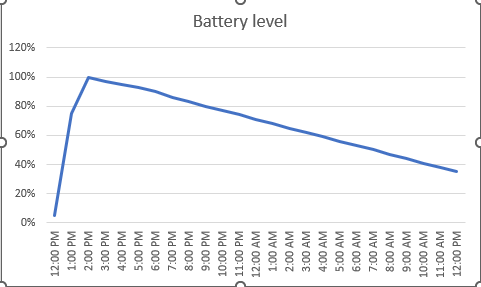
\includegraphics{battery_level}
  \\\textbf{Figure:}The battery levels in a span of 24 hours

  \item{\textbf{RT\_2: Battery Charge Protection}}\label{RT2}

  \textbf{Initial State}: Battery is fully charged.

  \textbf{Input}: Connect battery to the charging cable.

  \textbf{Expected Results}: Battery will not overcharge.

  Test Case Derivation: N/A

  \textbf{How test was performed}: Battery component was isolated from device and fully charged, then it wasn't unplugged and left around for couple minutes .

  \textbf{Observed Results}: Battery was not being overcharged nor did it heat up, thus device was safe to use.

\end{enumerate}

\subsection{Accuracy}
The following set of tests were executed to ensure that the device can recognize its state and perform its main functionality in accurate manner, based on the state.
The following functional requirements test cases are applicable for accuracy:

\begin{itemize}
  \item MTT\_1: \hyperref[MTT1]{Regular Movement}
  \item MTT\_2: \hyperref[MTT2]{Slow Movement}
  \item PRT\_1: \hyperref[PRT1]{Test Prompt}
  \item PRT\_2: \hyperref[PRT2]{Activity Prompt}
\end{itemize}

\subsubsection{Usability}
The following set of tests were done to ensure that the device is usable by target user population is not problematic in terms of maintenance and user interactions.
\begin{enumerate}

  \item\textbf{{UT\_1: Intuitive UI\\}}\label{UT1}

  \textbf{Initial State}: The device is turned on and a question prompt is generated on screen.

  \textbf{Input}: Testers are asked to answer the questionnaire set without assistance in less than 1 minute.
  \textbf{Expected Results}: All testers are able to answer their prompt successfully.

  \textbf{How test was performed}: A test group of people with age of 40 or older was be asked to receive a powered-on EMAnator and asked to respond to a set of 3 questions in 1 minute. These questions were randomly selected from the following 10 questions.

  \begin{itemize}
    \item Are you a dog person or a cat person?
    \item Are you currently inside of a building?
    \item Are you currently a student?
    \item Did you make your bed this morning?
    \item Do you feel tired right now?
    \item Do you prefer coffee or tea?
    \item Do you have a G driver's license?
    \item Do you feel sleepy right now?
    \item Which is better: Summer vs Winter
    \item Is it daytime right now?
  \end{itemize}

  \textbf{Observed Results}: The UI was very intuitive and user-friendly. Volunteers were able to navigate through and answer propmpts with ease.

  \item\textbf{{UT\_2: Comfortable Device\\}}\label{UT2}

  \textbf{Initial State}: The device is turned on and left on idle mode.

  \textbf{Input}: Testers are asked to wear the device for 24 hours.

  \textbf{Expected Results}: Testers fill out a survey form regarding the comfort of the device on their body.

  \textbf{How test was performed}: At the end of their 1 day cycle, testers will be asked to fill out an online form indicating how comfortable they felt the device was regards to weight, shape, stability, etc. The following questions will be asked.

  \begin{itemize}
    \item Did the device every fall off? If so, please record the following for each case: What you were doing each time? When did the incident happen?
    \item How do you feel regarding the weight of the device? Was it too heavy or too light?
    \item How do you feel regarding the texture of the device? Did you find it uncomfortable in any way?
  \end{itemize}

  \textbf{Observed Results}: Testers filled out a survey and the responses were mostly positive.

  \item\textbf{{UT\_3: Reusability\\}}\label{UT3}

  \textbf{Initial State}: The device is cleaned using isopropyl alcohol wipes.

  \textbf{Input}: Testers visually inspect how clean the device is.

  \textbf{Expected Results}: The device is deemed clean and the device is not harmed.

  \textbf{How test was performed}: A member of Back End Developers cleaned the device, which was later inspected for safety and usage to check if the device turned on and functioned normally.

  \textbf{Observed Results}: The device was functionally as normal despite being cleaned after usage.

\end{enumerate}

\subsubsection{Performance}
The following set of questions was asked to ensure that the device was capable of meeting user expectations.
\begin{enumerate}
  \item\textbf{{PT\_1: Data Transfer Time\\}}\label{PT1}

  \textbf{Initial State}: The device has collected a complete set of data.

  \textbf{Input}: The device is connected to the host software and connection is established for data transfer.

  \textbf{Expected Results}: Data transfer to finish within the specified parameter, TRANSFER\_TIME.

  \textbf{How test was performed}: 2 group members of the Back End Developers performed seperate data transfer tests 4 times and recorded the total transfer time for each execution. All 8 tests should result in execution time less than or equal to TRANSFER\_TIME.

  \textbf{Observed Results}: The data was transferred within the specified parameter, thus indicating device performed well in terms of transfer rates.

TRANSFER\_TIME: Set to 60 seconds

\begin{table}[H]
  \begin{tabular}{| c | c | m{3cm} | m{1.75cm} | m {5cm} |}
\hline
    \textbf{File Size} & \textbf{Transfer Time} & \textbf{Errors} & \textbf{Test Result} & \textbf{Notes }\\
\hline
2kB & 2.66s & None & Pass & None \\
\hline
10kB& 13.27s & None & Pass & None \\
\hline
8.5kB& 10.51s & None & Pass & None \\
\hline
5kB& 6.94s & None & Pass & None \\
\hline
11kB& 14.10s & None & Pass & None \\
\hline
18kB & N/A & COM Port 7 Not Open & Result Rejected & Cable was plugged in incorrectly. \\
\hline
20kB & 25.68s & None & Pass & None \\
\hline
35kB & 36.85s & None & Pass & None \\
\hline
  \end{tabular}
\caption{Data Transfer Time Testing Data}
\end{table}

  \item\textbf{{PT\_2: Battery Life\\}}\label{PT2}

  \textbf{Initial State}: The device is turned on and left on idle mode.

  \textbf{Input}: Testers wear the device for standard monitoring period.

  \textbf{Expected Results}: The total amount of time before the device runs out of battery is greater or equal to the parameter, BATTERY\_LIFE.

  \textbf{How test was performed}: 2 group members of the Back End Developers wore the device for standard monitoring period consecutively in their daily basis. At the end of each calendar day, they are prompted to record their response to a simple question: "Does the device still have battery life left?".

  \textbf{Observed Results}: The group members answered the prompt, thus giving us the time limit on the batteries. It was greater than the parameter set.

Minimum Battery Life: 24 Hours

\begin{table}[H]
  \begin{tabular}{| c | c | c | c | c |}
\hline
    \textbf{Battery Level} & \textbf{Errors} & \textbf{Prompt Response} & \textbf{Notes }\\
\hline
22\% & None & "Yes" & None \\
\hline
31\% & None & "Yes" & None \\
\hline
  \end{tabular}
\caption{Battery Performance Testing Data}
\end{table}

\end{enumerate}

\subsubsection{Data Security Tests}

These tests were designed to test the security of the system and the accessibility of important medical records. This is important to protect the user's privacy by avoiding it to fall in the wrong hands. Thus only authorised users can access the data.

\begin{enumerate}

  \item{\textbf{DSQT\_1: Records Safety Test}}\label{DSQT1}

  \textbf{Initial State}: Device is powered on.

  \textbf{Input}: Data transfer cable is plugged in from device to a generic PC, a volunteer tries to access the database and modify the data within.

  \textbf{Expected Results}: Database inaccessible and requests an administrative security key. The volunteer should be unable to access or modify the data.

  Test Case Derivation: N/A

  \textbf{How test was performed}: Device was given to a volunteer with required technical skills who did not have the administrator security key. They attempted to access the database.

  \textbf{Observed Results}: Databases couldn't be accessed and was prompting for a security key, implying the database is safe.

\end{enumerate}


\section{Comparison to Existing Implementation}
Current motion detecting smart watches, such as Apple watches or Samsung Galaxy watches, are desgined for healthy and active population. The EMAnator is specifically geared towards older adults who have chronical back pain. Therefore, it is desgined to capture minor and subtle movements accurately.

\section{Unit Testing}

\begin{center}
\begin{table} 
\begin{tabular}{ | p{0.5cm} | p{2.8cm} |  p{1.1cm} | p{2.7cm} | p{2.7cm} | p{2.7cm} | p{1.1cm} |}
\hline
\textbf{No.} & \textbf{Name}  & \textbf{Ref.} & \textbf{Action} & \textbf{Expected Output} & \textbf{Actual Output} & \textbf{Result} \\
\hline
 1 & bed\_HR\_setup & \href{https://github.com/zakerl/Capstone_Project/blob/main/docs/SRS/SRS.pdf}{R2} & Power on the device. & "PulseSensor object created", LED flash per each heartbeat. & "PulseSensor object created", LED flash per each heartbeat. & Pass \\ 
\hline
2 & bed\_HR\_detect & \href{https://github.com/zakerl/Capstone_Project/blob/main/docs/SRS/SRS.pdf}{R2} & Walk for 10 seconds while wearing the device, then stop. & "HeartBeat Detected. BPM: 70”. & "HeartBeat Detected. BPM: 130”. & Fail \\  
\hline
3 & bed\_MPU\newline \_setup & \href{https://github.com/zakerl/Capstone_Project/blob/main/docs/SRS/SRS.pdf}{R2} & Power on the device. & “Calibrating MPU in 4 seconds! Hold it still! avg X acc: 20, , avg Y acc: 20, avg Z acc: 20” & “Calibrating MPU in 4 seconds! Hold it still! avg X acc: 20, , avg Y acc: 20, avg Z acc: 20” & Pass \\  
\hline
4 & bed\_MPU\newline \_detect & \href{https://github.com/zakerl/Capstone_Project/blob/main/docs/SRS/SRS.pdf}{R2} & Limp & “limp count + limp count + limp count + limp count + limp count + limping. Stepcount: 5” & “limp count + limp count + limp count + limp count + limp count + limping. Stepcount: 5” & Pass \\ 
\hline
5 & bed\_init\_display & \href{https://github.com/zakerl/Capstone_Project/blob/main/docs/SRS/SRS.pdf}{NFR2} & Action & Black screen on & Black screen on & Pass \\ 
\hline
6 & bed\_scroll\_test &  \href{https://github.com/zakerl/Capstone_Project/blob/main/docs/SRS/SRS.pdf}{NFR2} & Scroll through 2 bezels in counter clock-wise direction. & Selection goes up. & Selection goes up. & Pass \\ 
\hline
7 & bed\_splash\newline \_screen & \href{https://github.com/zakerl/Capstone_Project/blob/main/docs/SRS/SRS.pdf}{NFR2} & Power on the device. & "Back End Developers" & "Back End Developers" & Pass \\ 
\hline
8 & bed\_display\newline \_one\_line & \href{https://github.com/zakerl/Capstone_Project/blob/main/docs/SRS/SRS.pdf}{NFR2} & Select a response for generated prompt & Screen clears prompt list and only displays current date and time. & Screen clears prompt list and only displays current date and time. & Pass \\ 
\hline
9 & OpenFile & \href{https://github.com/zakerl/Capstone_Project/blob/main/docs/SRS/SRS.pdf}{R6} & Press button and choose the "data.txt" file. & Contents of "data.txt" is displayed on UI. & Contents of "data.txt" is displayed on UI.  & Pass \\ 
\hline
\end{tabular}
\end{table}
\end{center}

\begin{center}
\begin{table} 
\begin{tabular}{ | p{0.5cm} | p{2.8cm} |  p{1.1cm} | p{2.7cm} | p{2.7cm} | p{2.7cm} | p{1.1cm} |}
\hline
\textbf{No.} & \textbf{Name}  & \textbf{Ref.} & \textbf{Action} & \textbf{Expected Output} & \textbf{Actual Output} & \textbf{Result} \\
\hline
10 & bed\_display\newline \_prompt & \href{https://github.com/zakerl/Capstone_Project/blob/main/docs/SRS/SRS.pdf}{R3} & Move around for 5 seconds and then stop for 5 seconds. & "Are you in pain?", Yes, No & "Are you in pain?", Yes, No & Pass \\ 
\hline
11 & bed\_format\newline \_prompt & \href{https://github.com/zakerl/Capstone_Project/blob/main/docs/SRS/SRS.pdf}{R3} & Limp with the device to activate prompt generation. & Prompt text color is white while background is black. & Prompt text color is white while background is black.  & Pass \\ 
\hline
12 & OpenSerial & \href{https://github.com/zakerl/Capstone_Project/blob/main/docs/SRS/SRS.pdf}{R6, NFR14} & Connect device to computer via USB port. & UI displays green dot. & UI displays green dot. & Pass \\ 
\hline
13 & bed\_init\_rtc & \href{https://github.com/zakerl/Capstone_Project/blob/main/docs/SRS/SRS.pdf}{R6, NFR1} & Power on the device. & "March 5th, 16:21". & "March 5th, 16:21". & Pass \\ 
\hline
14 & bed\_display\_info & \href{https://github.com/zakerl/Capstone_Project/blob/main/docs/SRS/SRS.pdf}{NFR2} & Power on the device. & "March 5th, 16:23". & "March 5th, 16:23". & Pass \\ 
\hline
15 & bed\_set\newline \_explicit\_date\newline \_time & \href{https://github.com/zakerl/Capstone_Project/blob/main/docs/SRS/SRS.pdf}{R6, NFR1} & Disconnect power source, reconnect, and power on the device. & "March 5th, 16:46". & "March 5th, 16:46". & Pass \\ 
\hline
16 & bed\_touch\newline \_detect & \href{https://github.com/zakerl/Capstone_Project/blob/main/docs/SRS/SRS.pdf}{NFR2} & Touch 2 bezels in clockwise direction. & 1 & 1 & Pass \\ 
\hline
17 & \_\_init\_\_ & N/A & Run the host software. & Login page appears. & Login page appears. & Pass \\ 
\hline
18 & saveAsTxt & \href{https://github.com/zakerl/Capstone_Project/blob/main/docs/SRS/SRS.pdf}{R6} & Press Save as button and choose a directory to save file in. & Config.txt file created and saved. & Config.txt file created and saved. & Pass \\ 
\hline
19 & BackToMain & \href{https://github.com/zakerl/Capstone_Project/blob/main/docs/SRS/SRS.pdf}{NFR2} & Press the main button. & Main screen appears and current screen closes. & Main screen appears and current screen closes. & Pass \\ 
\hline
20 &  InsertDB & \href{https://github.com/zakerl/Capstone_Project/blob/main/docs/SRS/SRS.pdf}{R6, NFR14} & Press save button. & Data appears on database table. & Data appears on database table. & Pass \\ 
\hline
\end{tabular}
\end{table}
\end{center}

\begin{center}
\begin{table} 
\begin{tabular}{ | p{0.5cm} | p{2.8cm} |  p{1.1cm} | p{2.7cm} | p{2.7cm} | p{2.7cm} | p{1.1cm} |}
\hline
\textbf{No.} & \textbf{Name}  & \textbf{Ref.} & \textbf{Action} & \textbf{Expected Output} & \textbf{Actual Output} & \textbf{Result} \\
\hline
21 & LoadDb & \href{https://github.com/zakerl/Capstone_Project/blob/main/docs/SRS/SRS.pdf}{R6, NFR14} & Press load button. & Data appears on software UI table. &  Data appears on software UI table. & Pass \\ 
\hline
22 & dataHead & \href{https://github.com/zakerl/Capstone_Project/blob/main/docs/SRS/SRS.pdf}{R6, NFR14} & Press load button. & Data appears on software UI table. & Data appears on software UI table. & Pass \\ 
\hline
23 & search & \href{https://github.com/zakerl/Capstone_Project/blob/main/docs/SRS/SRS.pdf}{R6, NFR14} & Filter-search participant first name of “John” & All participant record with first name “John” appears. & All participant record with first name “John” appears. & Pass \\ 
\hline
24 & OpenGraph & \href{https://github.com/zakerl/Capstone_Project/blob/main/docs/SRS/SRS.pdf}{R7} & Press graph button. & Empty graph chart appears. & Empty graph chart appears. & Pass \\ 
\hline
25 & OpenHeart & \href{https://github.com/zakerl/Capstone_Project/blob/main/docs/SRS/SRS.pdf}{R7} & Press heart rate button. & Only heart rate graph appears. & Only heart rate graph appears. & Pass \\ 
\hline
26 & OpenSteps & \href{https://github.com/zakerl/Capstone_Project/blob/main/docs/SRS/SRS.pdf}{R7} & Press steps button. & Only number-of-steps graph appears. & Only number-of-steps graph appears. & Pass \\ 
\hline
27 & OpenActivity & \href{https://github.com/zakerl/Capstone_Project/blob/main/docs/SRS/SRS.pdf}{R7} & Press activity button & Only activity graph appears. & Only activity graph appears. & Pass \\ 
\hline
28 & plot & \href{https://github.com/zakerl/Capstone_Project/blob/main/docs/SRS/SRS.pdf}{R7} & Press steps button. & Only number-of-steps graph appears. & Only number-of-steps graph appears. & Pass \\ 
\hline
29 & loginAttempt & \href{https://github.com/zakerl/Capstone_Project/blob/main/docs/SRS/SRS.pdf}{NFR8, NFR14} & ID: "admin", PW: "capstone" & Main screen appears. & Main screen appears. & Pass \\ 
\hline
30 & loginAttempt & \href{https://github.com/zakerl/Capstone_Project/blob/main/docs/SRS/SRS.pdf}{NFR8, NFR14} & ID: "wr1ong", PW: "creden5tials" & "Wrong credentials!" & "Wrong credentials!" & Pass \\ 
\hline
31 & showRecord\newline Window & \href{https://github.com/zakerl/Capstone_Project/blob/main/docs/SRS/SRS.pdf}{NFR2} & Press records button. & Records window appears and main window closes. & Records window appears and main window closes. & Pass \\ 
\hline
32 & showCreate\newline Records & \href{https://github.com/zakerl/Capstone_Project/blob/main/docs/SRS/SRS.pdf}{NFR2} & Press create records button. & Create Records window appears and main window closes. & Create Records window appears and main window closes. & Pass \\ 
\hline
\end{tabular}
\end{table}
\end{center}

\begin{center}
\begin{table} 
\begin{tabular}{ | p{0.5cm} | p{2.8cm} |  p{1.1cm} | p{2.7cm} | p{2.7cm} | p{2.7cm} | p{1.1cm} |}
\hline
\textbf{No.} & \textbf{Name}  & \textbf{Ref.} & \textbf{Action} & \textbf{Expected Output} & \textbf{Actual Output} & \textbf{Result} \\
\hline
33 & showConfig\newline View & \href{https://github.com/zakerl/Capstone_Project/blob/main/docs/SRS/SRS.pdf}{NFR2} & Press configuration button. & Configuration window appears and main window closes. & Configuration window appears and main window closes. & Pass \\ 
\hline
34 & showDataView & \href{https://github.com/zakerl/Capstone_Project/blob/main/docs/SRS/SRS.pdf}{NFR2} & Press data view button. & Data view window appears and main window closes. & Data view window appears and main window closes. & Pass \\ 
\hline
\end{tabular}
\end{table}

\end{center}

\section{Changes Due to Testing}

After testing out each unit of the device system and failing unit test \#2, the type of heartrate sensor has been changed. Below table outlines the rejected heartrate sensor candidates for EMAnator.


\textbf{Heart Rate Sensor Options:}\\

\begin{table}[H]

  \label{HRSensors_Pt1}\caption{Tested Heart Rate Sensors Part 1}
  \begin{tabular}{ | c | m{3cm} | c | m{7cm} |}
    \hline
    \textbf{Image}                              & \textbf{Model}                                                                                                                                                    & \textbf{Status} & \textbf{Reason for Status}                                                                                                                                                                                                                                               \\
    \hline
    See Figure \ref{fig:G21394}    & \href{https://secure.sayal.com/STORE2/View_SHOP.php?SKU=247799}{Chaney Electronics Inc. G21394}                                                                   & Rejected        & Due to the Infrared LED's Placement and the photoelectic sensor's placement, it is impossible to integrate the module with a device sitting on the wrist.                                                                                                                \\
    \hline
    See Figure \ref{fig:sparkfun}     & \href{https://www.sparkfun.com/products/15219}{SparkFun Pulse Oximeter and Heart Rate Sensor - MAX30101 \& MAX32664 (Qwiic)}                                      & Rejected        & Chronically out of stock, and requires extra complexity to be built into the PCB in order for this to function.                                                                                                                                                          \\
    \hline
    See Figure \ref{fig:grove1}      & \href{https://www.seeedstudio.com/Grove-Finger-clip-Heart-Rate-Sensor.html?queryID=ad9334e40c7058a87ffd810044eecd1c                                               & objectID=711    & indexName=bazaar_retailer_products}{Grove - Finger-clip Heart Rate Sensor}                                                                                & Rejected & Size too large, and issues with skin contact to the sensor results in garbage data.               \\
    \hline
    See Figure \ref{fig:grove2}      & \href{https://www.seeedstudio.com/Grove-Ear-clip-Heart-Rate-Sensor.html?queryID=ad9334e40c7058a87ffd810044eecd1c                                                  & objectID=2143   & indexName=bazaar_retailer_products}{Grove - Ear-clip/Finger-clip Heart Rate Sensor}                                                                       & Rejected & Sensor attachment to the ear was considered too disruptive to the participant's daily activities. \\
    \hline
    See Figure \ref{fig:knockoff}     & \href{https://www.amazon.ca/Comimark-Sensor-Module-Arduino-Raspberry/dp/B07V6VV8CM}{Comimark 2Pcs Heart Rate Pulse Sensor Sensor Module for Arduino Raspberry pi} & Rejected        & Build quality was unacceptably bad. Ordered name-brand version of this product next.                                                                                                                                                                                     \\                                                                                              \\
    \hline
    See Figure \ref{fig:pulseSensor} & \href{https://pulsesensor.com/}{PulseSensor.com Pulse Sensor}                                                                                                     & Accepted        & Build quality was better than knock-offs from before. Skin contact issue still present, but attempts are being made to solve this issue using software.                                                                                                                  \\
    \hline
  \end{tabular}
\end{table}

\begin{figure}[H]
  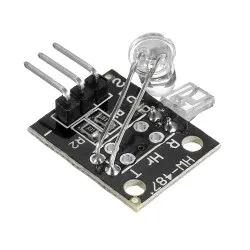
\includegraphics[scale=1]{G21394}
  \caption{Chaney Electronics Inc. G21394}
  \label{fig:G21394}
\end{figure}

\begin{figure}[H]
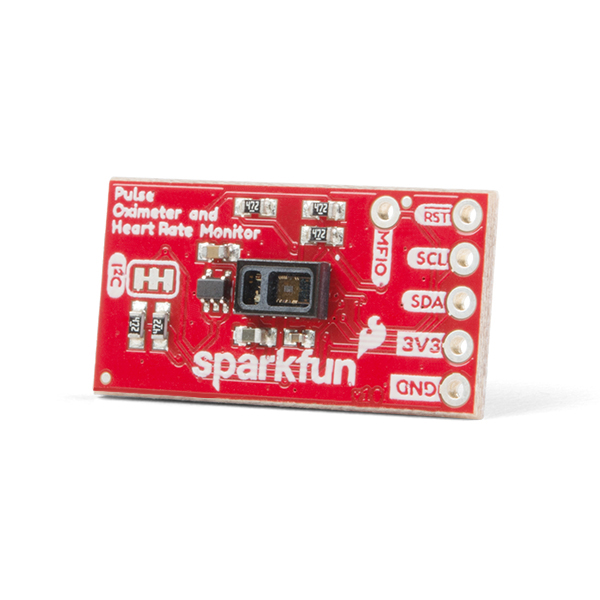
\includegraphics[scale = 1]{sparkfun} 
  \caption{SparkFun Pulse Oximeter and Heart Rate Sensor - MAX30101 \& MAX32664 (Qwiic)}
  \label{fig:sparkfun}
\end{figure}

\begin{figure}[H]
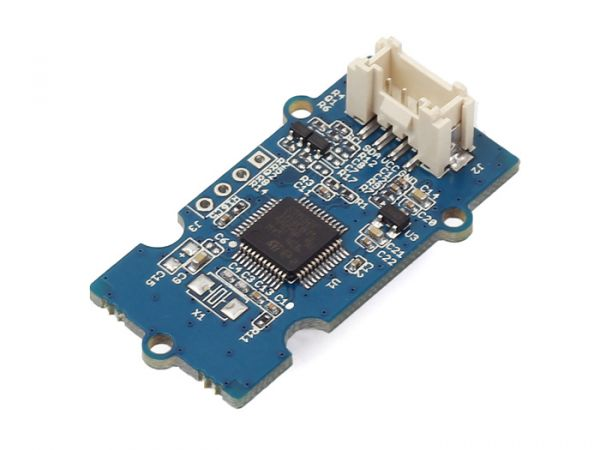
\includegraphics[scale = 0.5]{grove1}
  \caption{Grove - Finger-clip Heart Rate Sensor}
  \label{fig:grove1}
\end{figure}

\begin{figure}[H]
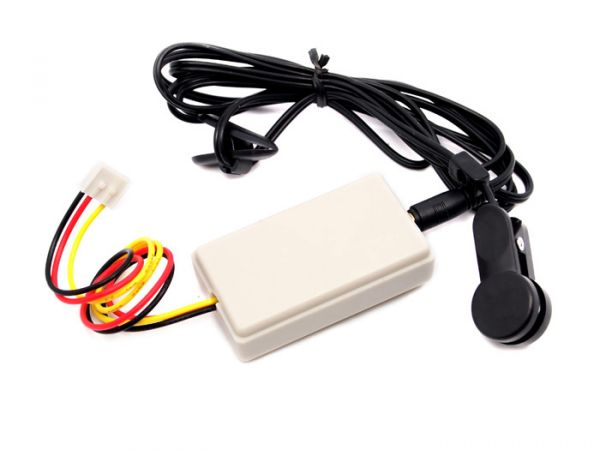
\includegraphics[scale = 0.5]{grove2}
  \caption{Grove - Ear-clip/Finger-clip Heart Rate Sensor}
  \label{fig:grove2}
\end{figure}

\begin{figure}[H]
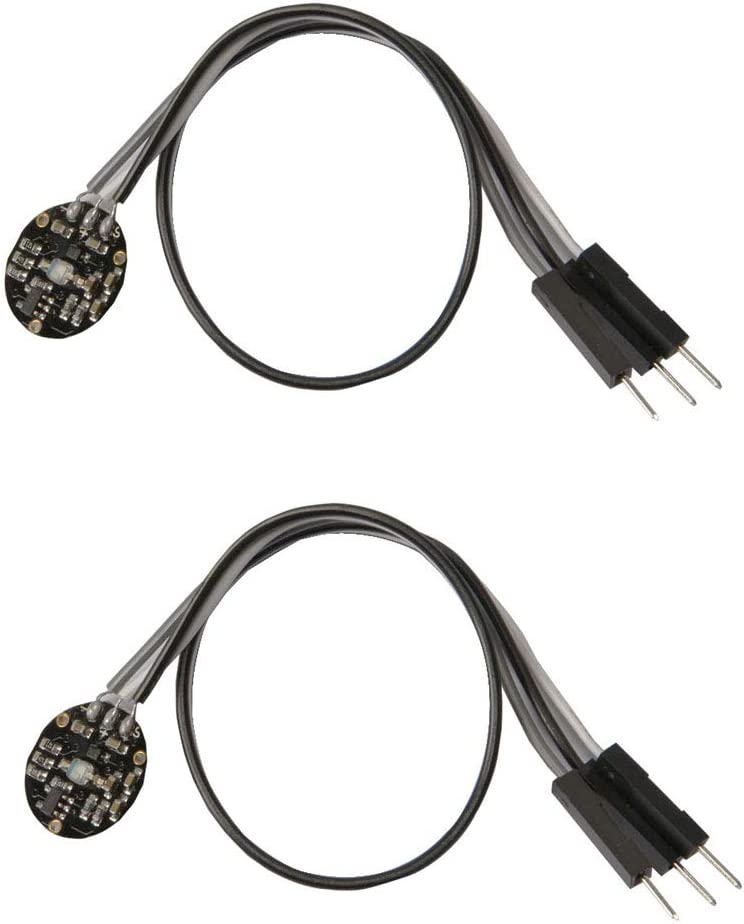
\includegraphics[scale = 0.25]{knockoff}
  \caption{Comimark 2Pcs Heart Rate Pulse Sensor Sensor Module for Arduino Raspberry pi}
  \label{fig:knockoff}
\end{figure}

\begin{figure}[H]
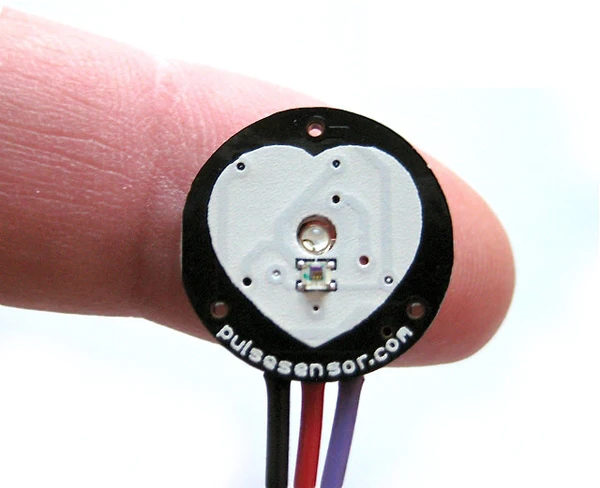
\includegraphics[scale = 0.5]{pulseSensor}
  \caption{PulseSensor.com Pulse Sensor}
  \label{fig:pulseSensor}
\end{figure}

\textbf{Last Minute Change to Microcontroller}

A major change to the design was a last minute switch to the ESP32 microcontroller after originally working with the Seeedunio Xiao microcontroller until Revision 0. The decision to switch had to be made for reasons explained below. But, unfortunately this change was only made after significant progress had already been made by the Back End Developers. Going as far as designing and printing a custom PCB with all required hardware and sensors, and integrating the codebase with the Seeeduino Xiao and PCB prior to the Revision 0 demonstration. \\

The Seeedunio Xiao was originally chosen because it runs on a similar ARM based platform compared to the Arduino Nano which was used for testing. This made development easier and provided enough processing power to meet the needs of the design. The Seeduino SAMD21 Cortex M0+ chip has as clock speed of 48 MHz which is 4x faster the clock speed on a typical Arduino Nano of 16 MHz. Additionally, the Seeeduino is a much smaller device than the Nano and could be directly soldered onto the 44mm diameter custom PCB. It would not take up significant space, leaving room for the rest of the sensors and hardware and allowing the design to fit within standard smartwatch dimensions. \\

During development and testing the Seeeduino did not present any issues and development was progressing well. However, leading up to the Revision 0 demo multiple Seeeduinos entered into an irrecoverable state. The reason for why this occurred is still unclear. However, after reading online the Back End Developers speculate two main reasons. First, it is possible that the bootloader region was not properly protected from the factory and it was accidentally overwritten by the software. Second, it is possible that there was not adequate power/surge protection for the Seeeduino since it seemed to fail some time after being connected to an external power supply for sensor testing but did not fail at all during use with a USB cable connected to a computer. \\

After more troubleshooting online it was discovered that this failure is a somewhat well documented issue with no easily available solution. This left the Back End Developers with no choice but to find an alternative microcontroller that did not have a major design flaw and would still meet the needs and constraints of the design. The alternative microcontroller that was chosen was the ESP32. The ESP can also run the Back End Developers code which reduces the total amount of refactoring that needs to be done. However, the pinout and size of the device differs from the Seeeduino meaning that the new custom PCB has to be made larger and the routing updated. The expected fabrication and shipping time will take over 1 week based on prior experience. \\

Due to the size and nature of the problem that was discovered at such a late stage in the project, there is a risk to the completion of the project as a whole. The time to integrate all the sensor code, display code and database code will be very limited once the new PCB arrives. Additionally, there is a risk that the PCB design does not perform the required functionality in the way that was intended. With a lead time of over 1 week if the PCB does not function as required the Back End Developers will have to fall back on a design that focuses on proof of concept rather than a fully fleshed out prototype. The proof of concept design will include functionality of sensing movement, prompting the user, collecting data, and enabling the researcher to view the data as intended by the functional requirements. \\

\section{Automated Testing}
N/A

\section{Trace to Requirements}

\noindent
\begin{table}[H]
  \centering
  \begin{tabular}{|c|c|c|c|c|c|c|c|c|c|}
    \hline
                   & \hyperref[DT1]{DT1} & \hyperref[DT2]{DT2} & \hyperref[DT3]{DT3} & \hyperref[DT4]{DT4} & \hyperref[MTT1]{MTT1} & \hyperref[MTT2]{MTT2} & \hyperref[PRT1]{PRT1} & \hyperref[PRT2]{PRT2} & \hyperref[TT1]{TT1} \\
    \hline
    \textbf{R1}    & X                   & X                   & X                   & X                   &                       &                       &                       &                       &                     \\ \hline
    \textbf{R2}    &                     &                     &                     &                     & X                     & X                     &                       &                       &                     \\ \hline
    \textbf{R3}    &                     &                     &                     &                     &                       &                       & X                     & X                     &                     \\ \hline
    \textbf{R4}    &                     &                     &                     &                     &                       &                       &                       &                       & X                   \\ \hline
    \textbf{R5}    &                     &                     &                     &                     &                       &                       &                       &                       &                     \\ \hline
    \textbf{R6}    &                     &                     &                     &                     &                       &                       &                       &                       &                     \\ \hline
    \textbf{NFR1}  &                     &                     &                     &                     & X                     & X                     & X                     & X                     &                     \\ \hline
    \textbf{NFR12} &                     &                     &                     &                     &                       &                       & X                     &                       &                     \\ \hline
  \end{tabular}
  \caption{ Requirements Traceability Matrix Pt1}
  \label{Table:A_Req_trace}
\end{table}



\begin{table}[H]
  \centering
  \begin{tabular}{|c|c|c|c|c|c|c|c|c|c|c|}
    \hline
                & \hyperref[TT2]{TT2} & \hyperref[TT3]{TT3} & \hyperref[TT4]{TT4} & \hyperref[TT5]{TT5} & \hyperref[DST1]{DST1} & \hyperref[DST2]{DST2} & \hyperref[DST3]{DST3} & \hyperref[DXT1]{DXT1} & \hyperref[DXT2]{DXT2} & \hyperref[DXT3]{DXT3} \\
    \hline
    \textbf{R1} &                     &                     &                     &                     &                       &                       &                       &                       &                       &                       \\ \hline
    \textbf{R2} &                     &                     &                     &                     &                       &                       &                       &                       &                       &                       \\ \hline
    \textbf{R3} &                     &                     &                     &                     &                       &                       &                       &                       &                       &                       \\ \hline
    \textbf{R4} & X                   & X                   & X                   & X                   &                       &                       &                       &                       &                       &                       \\ \hline
    \textbf{R5} &                     &                     &                     &                     & X                     & X                     & X                     &                       &                       &                       \\ \hline
    \textbf{R6} &                     &                     &                     &                     &                       &                       &                       & X                     & X                     & X                     \\ \hline
  \end{tabular}
  \caption{Requirements Traceability Matrix Pt2}
  \label{Table:B_Req_trace}
\end{table}

\begin{table}[H]
  \centering
  \begin{tabular}{|c|c|c|c|c|c|c|c|c|c|c|c|}
    \hline
                   & \hyperref[HST1]{HST1} & \hyperref[HST2]{HST2} & \hyperref[HST3]{HST3} & \hyperref[HST4]{HST4} & \hyperref[RT1]{RT1} & \hyperref[UT1]{UT1} & \hyperref[UT2]{UT2} & \hyperref[UT3]{UT3} & \hyperref[PT1]{PT1} & \hyperref[PT2]{PT2} & \hyperref[DSQT1]{DSQT1} \\
    \hline
    \textbf{NFR2}  &                       &                       &                       &                       &                     & X                   & X                   & X                   &                     &                     &                         \\ \hline
    \textbf{NFR3}  &                       &                       &                       &                       &                     &                     &                     &                     &                     & X                   &                         \\ \hline
    \textbf{NFR4}  &                       &                       &                       &                       &                     &                     & X                   &                     &                     &                     &                         \\ \hline
    \textbf{NFR5}  &                       &                       &                       &                       &                     &                     &                     & X                   &                     &                     &                         \\ \hline
    \textbf{NFR6}  & X                     & X                     & X                     & X                     &                     &                     &                     &                     &                     &                     &                         \\ \hline
    \textbf{NFR7}  &                       &                       &                       &                       & X                   &                     &                     &                     &                     &                     &                         \\ \hline
    \textbf{NFR8}  &                       &                       &                       &                       &                     &                     &                     &                     &                     &                     & X                       \\ \hline
    \textbf{NFR9}  &                       &                       &                       &                       &                     & X                   &                     &                     &                     &                     &                         \\ \hline
    \textbf{NFR10} &                       &                       &                       &                       &                     &                     & X                   &                     &                     &                     &                         \\ \hline
    \textbf{NFR11} & X                     & X                     & X                     & X                     & X                   &                     &                     &                     &                     &                     &                         \\ \hline
    \textbf{NFR13} &                       &                       &                       &                       &                     &                     &                     &                     & X                   &                     &                         \\ \hline
    \textbf{NFR14} &                       &                       &                       &                       &                     &                     &                     &                     &                     &                     & X                       \\ \hline
  \end{tabular}
  \caption{Requirements Traceability Matrix Pt3}
  \label{Table:C_Req_trace}
\end{table}
\newpage

\section{Trace to Modules}

\noindent
\begin{table}[H]
  \centering
  \begin{tabular}{|c|c|c|c|c|c|c|c|c|c|}
    \hline
                 & \hyperref[DT1]{DT1} & \hyperref[DT2]{DT2} & \hyperref[DT3]{DT3} & \hyperref[DT4]{DT4} & \hyperref[MTT1]{MTT1} & \hyperref[MTT2]{MTT2} & \hyperref[PRT1]{PRT1} & \hyperref[PRT2]{PRT2} & \hyperref[TT1]{TT1} \\
    \hline
    \textbf{M1}  & X                   &                     &                     &                     &                       &                       &                       &                       &                     \\ \hline
    \textbf{M2}  &                     &                     &                     &                     &                       &                       &                       &                       & X                   \\ \hline
    \textbf{M3}  &                     &                     &                     &                     &                       &                       &                       &                       &                     \\ \hline
    \textbf{M4}  &                     &                     &                     &                     & X                     & X                     &                       & X                     &                     \\ \hline
    \textbf{M5}  &                     &                     &                     &                     &                       &                       & X                     & X                     &                     \\ \hline
    \textbf{M6}  &                     &                     &                     &                     &                       &                       & X                     & X                     &                     \\ \hline
    \textbf{M7}  & X                   & X                   & X                   & X                   &                       &                       &                       &                       &                     \\ \hline
    \textbf{M8}  &                     &                     &                     &                     &                       &                       &                       &                       &                     \\ \hline
    \textbf{M9}  &                     &                     &                     &                     &                       &                       &                       &                       & X                   \\ \hline
    \textbf{M10} &                     &                     &                     &                     & X                     & X                     &                       & X                     &                     \\ \hline
  \end{tabular}
  \caption{ Module Traceability Matrix Pt1}
  \label{Table:A_Mod_trace}
\end{table}



\begin{table}[H]
  \centering
  \begin{tabular}{|c|c|c|c|c|c|c|c|c|c|c|}
    \hline
                 & \hyperref[TT2]{TT2} & \hyperref[TT3]{TT3} & \hyperref[TT4]{TT4} & \hyperref[TT5]{TT5} & \hyperref[DST1]{DST1} & \hyperref[DST2]{DST2} & \hyperref[DST3]{DST3} & \hyperref[DXT1]{DXT1} & \hyperref[DXT2]{DXT2} & \hyperref[DXT3]{DXT3} \\
    \hline
    \textbf{M1}  &                     &                     &                     &                     &                       &                       &                       &                       &                       &                       \\ \hline
    \textbf{M2}  & X                   & X                   & X                   & X                   &                       &                       &                       & X                     & X                     & X                     \\ \hline
    \textbf{M3}  &                     &                     &                     &                     & X                     & X                     & X                     & X                     & X                     & X                     \\ \hline
    \textbf{M4}  &                     &                     &                     &                     & X                     & X                     & X                     & X                     & X                     & X                     \\ \hline
    \textbf{M5}  &                     &                     &                     &                     &                       &                       &                       &                       &                       &                       \\ \hline
    \textbf{M6}  &                     &                     &                     &                     & X                     & X                     & X                     &                       &                       &                       \\ \hline
    \textbf{M7}  &                     &                     &                     &                     &                       & X                     & X                     &                       &                       &                       \\ \hline
    \textbf{M8}  &                     &                     &                     &                     &                       &                       &                       &                       &                       &                       \\ \hline
    \textbf{M9}  & X                   & X                   & X                   & X                   &                       &                       &                       &                       &                       &                       \\ \hline
    \textbf{M10} &                     &                     &                     &                     &                       &                       &                       &                       &                       &                       \\ \hline
  \end{tabular}
  \caption{Module Traceability Matrix Pt2}
  \label{Table:B_Mod_trace}
\end{table}

\begin{table}[H]
  \centering
  \begin{tabular}{|c|c|c|c|c|c|c|c|c|c|c|c|c|}
    \hline
                 & \hyperref[HST1]{HST1} & \hyperref[HST2]{HST2} & \hyperref[HST3]{HST3} & \hyperref[HST4]{HST4} & \hyperref[RT1]{RT1} & \hyperref[RT2]{RT2} & \hyperref[UT1]{UT1} & \hyperref[UT2]{UT2} & \hyperref[UT3]{UT3} & \hyperref[PT1]{PT1} & \hyperref[PT2]{PT2} & \hyperref[DSQT1]{DSQT1} \\
    \hline
    \textbf{M1}  & X                     & X                     & X                     & X                     & X                   & X                   &                     &                     &                     &                     & X                   &                         \\ \hline
    \textbf{M2}  &                       &                       &                       &                       &                     &                     &                     &                     &                     & X                   &                     & X                       \\ \hline
    \textbf{M3}  &                       &                       &                       &                       &                     &                     &                     &                     &                     &                     &                     &                         \\ \hline
    \textbf{M4}  &                       &                       &                       &                       &                     &                     &                     &                     &                     &                     &                     &                         \\ \hline
    \textbf{M5}  &                       &                       &                       & X                     &                     &                     & X                   &                     &                     &                     &                     &                         \\ \hline
    \textbf{M6}  &                       &                       &                       &                       &                     &                     & X                   &                     &                     &                     &                     &                         \\ \hline
    \textbf{M7}  &                       &                       &                       & X                     &                     &                     &                     &                     &                     &                     &                     &                         \\ \hline
    \textbf{M8}  &                       &                       &                       &                       &                     &                     &                     &                     &                     &                     &                     &                         \\ \hline
    \textbf{M9}  &                       &                       &                       &                       &                     &                     &                     &                     &                     &                     &                     &                         \\ \hline
    \textbf{M10} &                       &                       &                       &                       &                     &                     & X                   & X                   &                     &                     &                     &                         \\ \hline
  \end{tabular}
  \caption{Module Traceability Matrix Pt3}
  \label{Table:C_Mod_trace}
\end{table}
\newpage

\section{Code Coverage Metrics}
N/A
%\bibliographystyle{plainnat}
%\bibliography{../../refs/References}

\newpage{}
\section*{Appendix --- Reflection}

The information in this section will be used to evaluate the team members on the
graduate attribute of Reflection.  Please answer the following question:\\	

\textit{In what ways was the Verification and Validation (VnV) Plan different
        from the activities that were actually conducted for VnV?  If there were
        differences, what changes required the modification in the plan?  Why did
        these changes occur?  Would you be able to anticipate these changes in future
        projects?  If there weren't any differences, how was your team able to clearly
        predict a feasible amount of effort and the right tasks needed to build the
        evidence that demonstrates the required quality?  (It is expected that most
        teams will have had to deviate from their original VnV Plan.)}

-In what ways was it different from the VnV Plan?\\

The process of developing this project from a concept to its current state has been a humbling experience. We (Team \#1: The Back End Developers) believed that we comprehensively covered the timeline of our project in the VnV Plan. \\

-If there were differences, what changes required modification\\
-Why did these changes occur?\\
-Reflect on the quality of the project in general\\
-Reflect on the areas that are yet to be improved\\
-Would you be able to anticipate these changes in future projects?\\

Rubric Goals: The verification and validation data is used to make valid conclusions about the project, in terms of its quality and areas that have been improved and are yet to be improved.  The connection between the data and the conclusions is clear.\\
Rubric Goals: The team reflects on the differences between the VnV plan and the VnV report in the Reflection Appendix.  It is obvious that the team took the exercise seriously and that they have gained an understanding that will help with future VnV planning.\\

\end{document}